\subsection{Codeausführung}

\begin{frame}
\begin{center}
	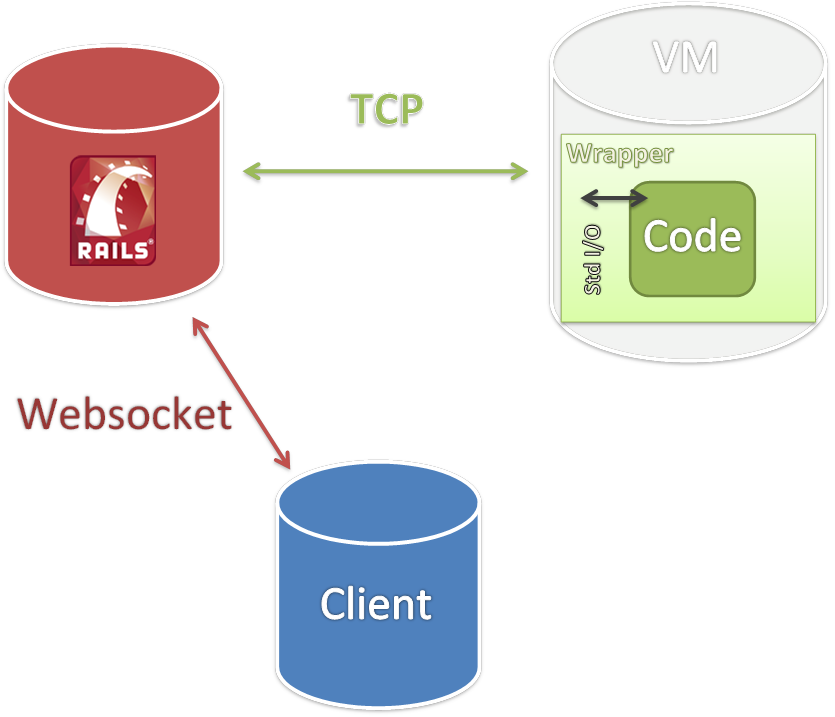
\includegraphics[scale=0.35]{overview}
\end{center}
\end{frame}

\begin{frame}
\frametitle{API}
\inputminted[linenos, numbersep=2pt, tabsize=4, frame=lines, label=move]{ruby}{vm/move.rb}
\end{frame}

\begin{frame}
\frametitle{API}
\inputminted[linenos, numbersep=2pt, tabsize=4, frame=lines, label=look]{ruby}{vm/look.rb}
\inputminted[linenos, numbersep=2pt, tabsize=4, frame=lines, label=response]{ruby}{vm/look_response.rb}
\end{frame}

\begin{frame}
\frametitle{Kommunikation mit der VM}
\begin{center}
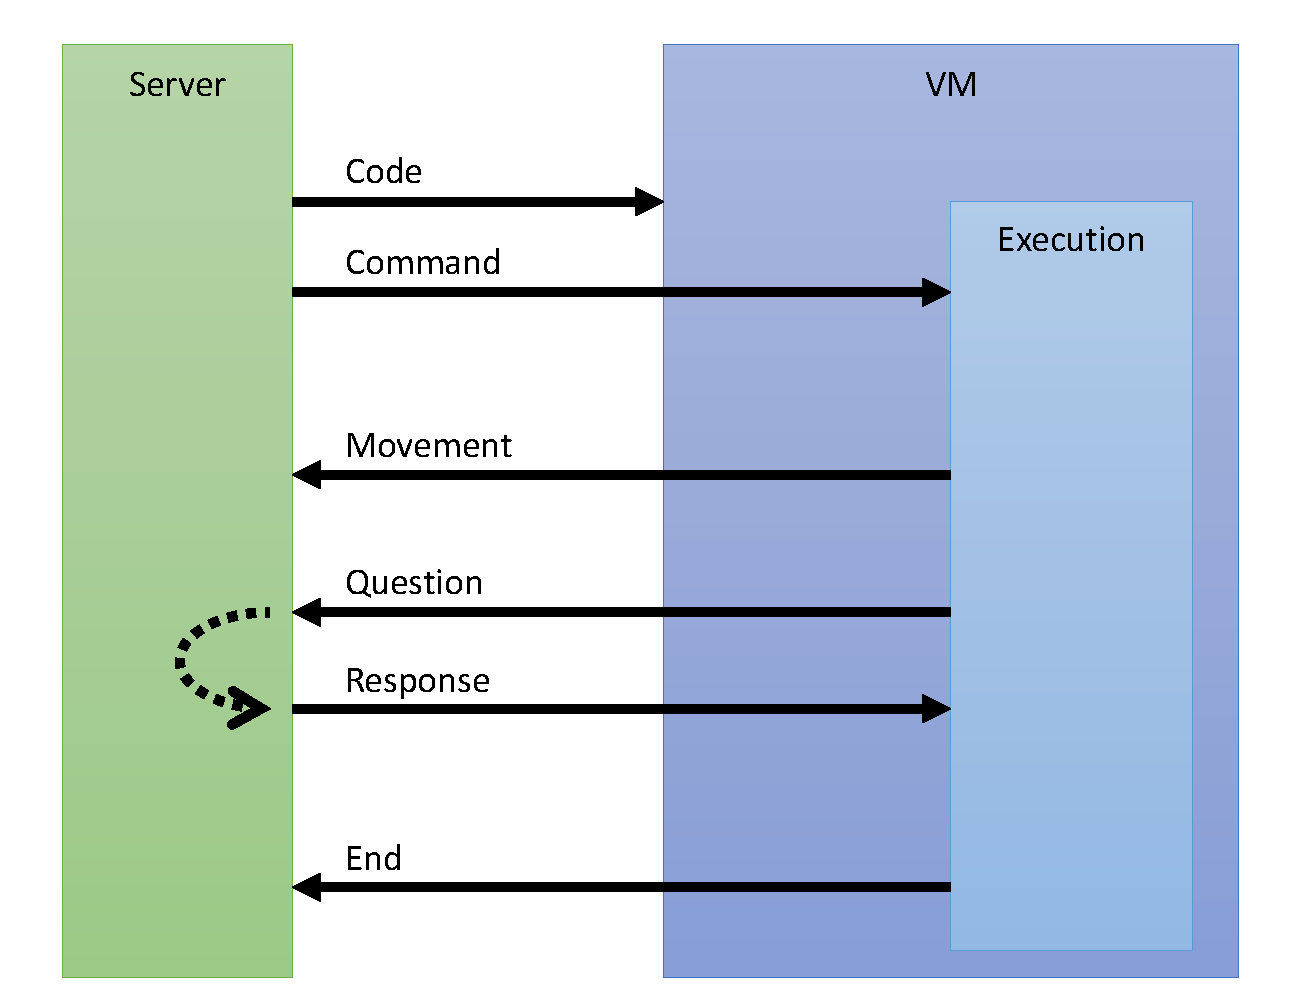
\includegraphics[width=250pt]{vm/vm.pdf}
\end{center}
\end{frame}